\documentclass[10pt]{article}

% Question: does spring constant of the stem or pencil matter?

\title{Drag on leaves in wind and flow-induced shape reconfiguration in grapefruit, {\emph{Citrus $\times$ paradisi}} (Rutaceae)}
\author{Cameron Smith\thanks{Author is with the Department of Weapons, Robotics, and Control Engineering at the United States Naval Academy. Address for correspondence: \emph{m226072@usna.edu}}}
\date{\today}


\usepackage[separate-uncertainty=true]{siunitx}
\DeclareSIUnit{\year}{y}
\DeclareSIUnit{\inch}{in}
\DeclareSIUnit{\foot}{ft}
\DeclareSIUnit{\poundforce}{lbf}
\DeclareSIUnit{\pound}{lbm}
\DeclareSIUnit{\frame}{frame}
\usepackage{graphicx}
\usepackage[round,authoryear]{natbib}
\bibliographystyle{apalike}
\usepackage[plain]{fancyref}
\usepackage{listings}
\usepackage{amsmath,amsfonts,amssymb}
\usepackage{booktabs}
\lstset{%
  basicstyle=\ttfamily,
  columns=fullflexible,
  showstringspaces=false}
\usepackage[dvipsnames,svgnames]{xcolor}
\usepackage{hyperref}
\hypersetup{%
  colorlinks=true,
  linkcolor=violet,
  urlcolor=blue,
  citecolor=blue}
\usepackage{svg}
%\usepackage{svg-extract}
\usepackage{fullpage}

\newcommand{\Citrusxparadisi}{\emph{Citrus $\times$ paradisi}}
\newcommand{\Cxparadisi}{\emph{C.~$\times$~paradisi}}
\newcommand{\Matlab}{Matlab}
\begin{document}

\maketitle
\begin{abstract}
This study was conducted to investigate how effectively citrus plants can change their structure to reduce drag in wind. Due to the COVID-19 outbreak, this study made use of an improvised flexure-based force sensor for drag. An elastic cord was attached to a young grapefruit (\Citrusxparadisi) plant and a rigid aluminum physical model of one of its leaves, in the presence of flow from a small fan.  Cord displacement was used to quantify drag, while the area normal to flow was obtained from image analysis using color thresholding and blob detection. The drag experienced by the rigid model was 19\% higher than the drag measured on the live plant. Slow motion video analysis indicated that this was the result of the citrus's ability to bend at the petiole. The extreme bending in several directions suggests a method of protective load shedding and may also indicate a potential way to avoid flow induced vibrational loads from vortex shedding.
\end{abstract}
{\scriptsize\textbf{Keywords: }grapefruit, \Citrusxparadisi, drag, leaf, petiole}

\section{Introduction}
Many organisms are subject to environmental flows and the forces that result from flow. Freely moving organisms may have to locomote in high wind or high currents; while sessile organisms may need to remain attached and undamaged during normal conditions as well as during extreme events \citep{vogel1994life, vogel2003comparative}. For example, interdal algae must remain attached to the bottom with a holdfast and must have stipes with sufficient mechanical strength for a variety of hydrodynamic loading conditions from drag and added mass \citep{carrington1992consequences, denny2002mechanics, stewart2004hydrodynamic, stewart2006hydrodynamic, boller2007interspecific}. Mechanistic models of forces may be combined with statistics of extreme events and measures of environmental safety factors to determine how long an organism or a community might be expected to persist in a particular environment \citep{denny2009on}. 

In the case of land plants, fluid forces from wind have important consequences for mechanical design \citep{delangre2008effects} as well as dispersal of seeds and pollen \citep{vogel2003comparative, evangelista2011explosive, stevenson2015when}. Wind can result in both lift and drag on a structure such as a plant; lift is transverse to the flow direction while drag is parallel with it \citep{vogel1994life, vogel2003comparative, kundu2012fluid}. Fluid flow over individual plants or within canopies creates drag on structures through pressure differences due to shape as well as friction in a thin boundary layer nearest the plant \citep{delangre2008effects, shapiro1961shape, kundu2012fluid, vogel1994life, vogel2003comparative}. If the drag exceeds some mechanical limit, the plant may experience mechanical failure by breaking or losing its attachment to the ground. 

Drag can be expressed as \citep{kundu2012fluid}:
\begin{equation}
D=0.5 C_D \rho V^2 A,
\label{eq:drag}
\end{equation}
where $D$ is the total drag force, $C_D$ is a nondimensional drag coefficient that is dependent on shape and on Reynolds number ($\operatorname{Re}$, a nondimensional ratio of inertial and viscous forces), $\rho=\SI{1.204}{\kilo\gram\per\meter\cubed}$ is the density of air, $V$ is relative fluid velocity, and $A$ is a reference area, here taken as the cross-sectional area of the surface normal to the flow direction. From \fref{eq:drag}, it is clear that $D$ can be minimized by reducing $C_D$ via changes in shape to a more streamlined form; reduction of $A$ via feathering into the wind, bending or curling of leaves \citep{ennos2000functional}, or sacrificial loss of branches to save the tree; and reduction of $V$ by bending/hunkering down in the boundary layer nearest the ground. Thus, plants can use their flexible structures to reconfigure under drag load, rolling their leaves into cones in order to minimize cross sectional area, drag coefficient, and the oscillations of vortex shedding \citep{miller2012reconfiguration, vogel1989drag, ennos2000functional}. This allows plants to endure the onslaught of heavy winds or floodwaters with much lower risk for structural damage than if they were to be entirely rigid. From an engineering point of view, these techniques are similar to feathering a propeller, reefing a sail, or protective load shedding in electrical systems.

In some cases, the interplay of elastic behavior of a flexible stem and the fluid mechanics as shape changes can result in dynamic flutter and other similar behaviors \citep{miller2012reconfiguration, boller2007interspecific, denny2002mechanics}. For the case of land plants, as shown in simulations by \citet{miller2012reconfiguration}, the presence of a flexible tether on the leaves, such as their stems, results in increased vortex shedding, causing much more erratic fluttering and increased drag forces. For this reason, plants vary in levels of rigidity in their leaf stems, in an effort to minimize drag while also avoiding excessive vortex shedding \citep{miller2012reconfiguration, vogel2009leaves}. 
    
Issues of plant response to high wind loads resulting in high drag are especially interesting in the case of tropical fruits, which are economically important and also grow natively in areas subject to hurricanes and cyclones. \citet{ennos2000functional} considered the mechanical role of the leaf petiole (the stem portion attaching at the proximate end of the leaf) in bananas (\emph{Musa textilis}) and found its U-shaped cross section allowed it sufficient flexural rigidity to hold up the broad leaves during normal conditions, but also provided sufficient torsional compliance to allow the leaves to feather into the wind during high loads. 
    
Another economically important tropical fruit with an interesting leaf petiole is the grapefruit, \Citrusxparadisi\ (Macfad.), whose winged petioles (\fref{fig:methods:specimens}) exhibit a peculiar jointed structure \citep{morton1987grapefruit, kumamoto1987mystery, macfayden1837flora}. It is possible that such a structure presents a balance between the counterproductive rigidity found by \citet{miller2012reconfiguration} as it combines the rigid nature of the petiole itself with the flexible nature of a joint. It may also constrain bending to certain preferential directions depending on the magnitude and direction of the wind loading on an individual leaf. The purpose of this study is to investigate the effectiveness of this petiole structure when compared to a structure lacking in all flexibility. I hypothesize that, compared to a rigid leaf, a live \Cxparadisi\ plant will bend and reconfigure its shape as flow increases, achieving lower drag either through static bending or through time-varying flutter processes that provide lower average force overall than the rigid condition. Due to the current COVID-19 outbreak, I will test my hypotheses by measuring forces with an elastic flexure-based apparatus \citep{denny1983simple, bell1984quantifying} on a live specimen compared with a rigid physical model \citep{stevenson2015when, evangelista2014shifts, stewart2006hydrodynamic, vogel2009leaves}. 

 %\section{Introduction}
\section{Methods and materials}
\begin{itemize}
\item 1 six-year old grapefruit plant
\item 1 cord of known spring constant
\item 1 measuring tape
\item 1 Kaz Inc. Ht-908 15 inch Honeywell Turbo Force Room Air Circulator Fan
\item colored construction paper
\item 1 pair of scissors
\item clear tape
\item 1 Samsung Galaxy S-8 smartphone camera
\item 1 wooden chair
\item flat, rectangular surfaces
\item MATLAB software
\item pipe cleaners
\item nylon rope
\end{itemize}

	The first step in the process was to find a cord of known spring constant. In this experiment, a cord from a party mask was found to have a spring coefficient of \SI{1.03}{\newton\per\centi\meter}. The cord was attached to a nylon rope and tied to pipe cleaners at both ends so that it could be connected to plant stems. The pipe cleaners were included in the spring constant calculation.

	The experimental setup for measuring the spring's deflection due to drag is shown in \fref{fig:methods1}. The cord was strung between a heavy chair and the trunk of a grapefruit plant so that it was not slack, and its length was measured using a tape measure. Then, a box fan was placed one foot away from the trunk of the plant. The plant and fan were raised using flat, rectangular objects, such as textbooks, in order to position the plant's canopy in front of the fan. The cord's deflection was measured five times at each of the fan's three speed settings and a slow motion video of the plant's leaves was taken at the highest fan setting.

Next, the cross sectional area of the plant was calculated using color blob detection in Matlab. To do this, black construction paper was cut to the size and shape of the fan's opening and affixed to it. Because air was blowing from relatively close to the plant, only the area which was directly in front of the fan opening would be exposed to wind. The plant was of a complex shape, so it was more efficient to calculate the area of the fan which was not covered by the plant. The setup was photographed from afar and scaled to eliminate the colorful surroundings, as shown in appendix~\ref{app:A}. A picture of the fan-shaped paper was also taken against a blue background from the same distance with no citrus obscuring it and scaled by the same amount, which can also be seen in appendix~\ref{app:A}. Using Matlab's \lstinline{colorThresholder} system, the ratio of covered to uncovered area was found and multiplied by the known paper area to find the area of the grapefruit leaves.

After analyzing the results of the grapefruit plant, a rigid model of a single leaf was created to test the same conditions without the presence of bending. A small leaf was placed against an aluminum Chipotle bowl lid to serve as a stencil, which was cut out using scissors. Then, this model leaf was taped to a wooden pencil so that the pencil would prevent it from flexing, while any tape edges were cut off. The finished leaf model can be seen in \fref{fig:methods2}. 

The leaf model was tested in the same manner as the grapefruit plant at the highest fan setting. Because the deflection in the cord was quite small, the displacement was measured using slow motion video. To do this, a tape measure with millimeters marked was taped below the cord and the video was taken from directly above. The video device was planted on a solid surface to minimize movement, and the displacement was found by zooming in on the video and pausing when the cord was fully extended and relaxed. The experimental setup for the model can be seen in \fref{fig:methods3}.

In order to compare the model area to the area of the grapefruit, a sheet of orange construction paper was photographed with and without the model leaf against it. Then, using the color blob detection technique in Matlab, the ratio of the model area to the paper area was calculated and multiplied by the actual paper area, in square feet. The images for this analysis can be seen in appendix~\ref{app:A}.

With the approximate cross sectional areas of the actual grapefruit leaves and the model found, the discussion over how these areas and their corresponding drags differed could begin.


% Fig 1 is good but cluttered, can we zoom in on only the business part; or turn it into a drawing. Altnatively, add callouts and scale bar? Is there a shot more from the side, that shows the experimental rig without foreshortening? 
% Agreed, I'll put in a drawing instead to make it neater
\begin{figure}
\begin{center}
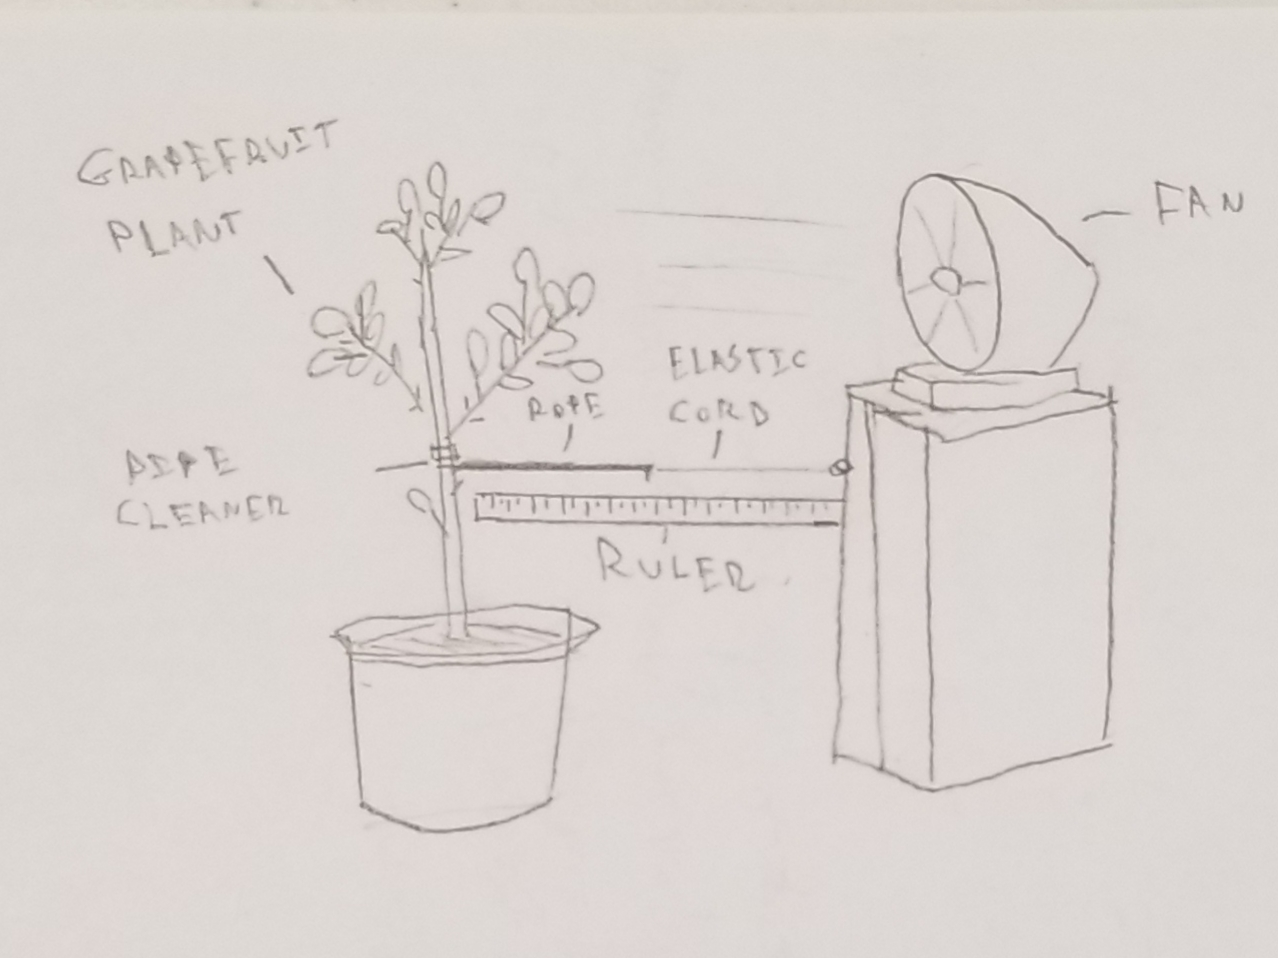
\includegraphics[width=0.5\columnwidth]{figures/Setup1.jpg} 
\end{center}
\caption{Experimental setup to measure the deflection of a grapefruit plant when exposed to wind.}
\label{fig:methods1}
\end{figure}

% Fig 2 is good but zoom in on the two, add callouts and a scalebar, maybe rotate leaves into their normal positions. 
\begin{figure}
\begin{center}
\includegraphics[width=0.33\columnwidth]{figures/Metal_Leaf_Compared.jpg}
\includegraphics[width=0.33\columnwidth]{figures/Measured Model.jpg}
\end{center}
\caption{The aluminum grapefruit leaf model (left) with a small jackfruit leaf. Measuring tape (cm) along the model, for scale (right).}
\label{fig:methods2}
\end{figure}

\begin{figure}
\begin{center}
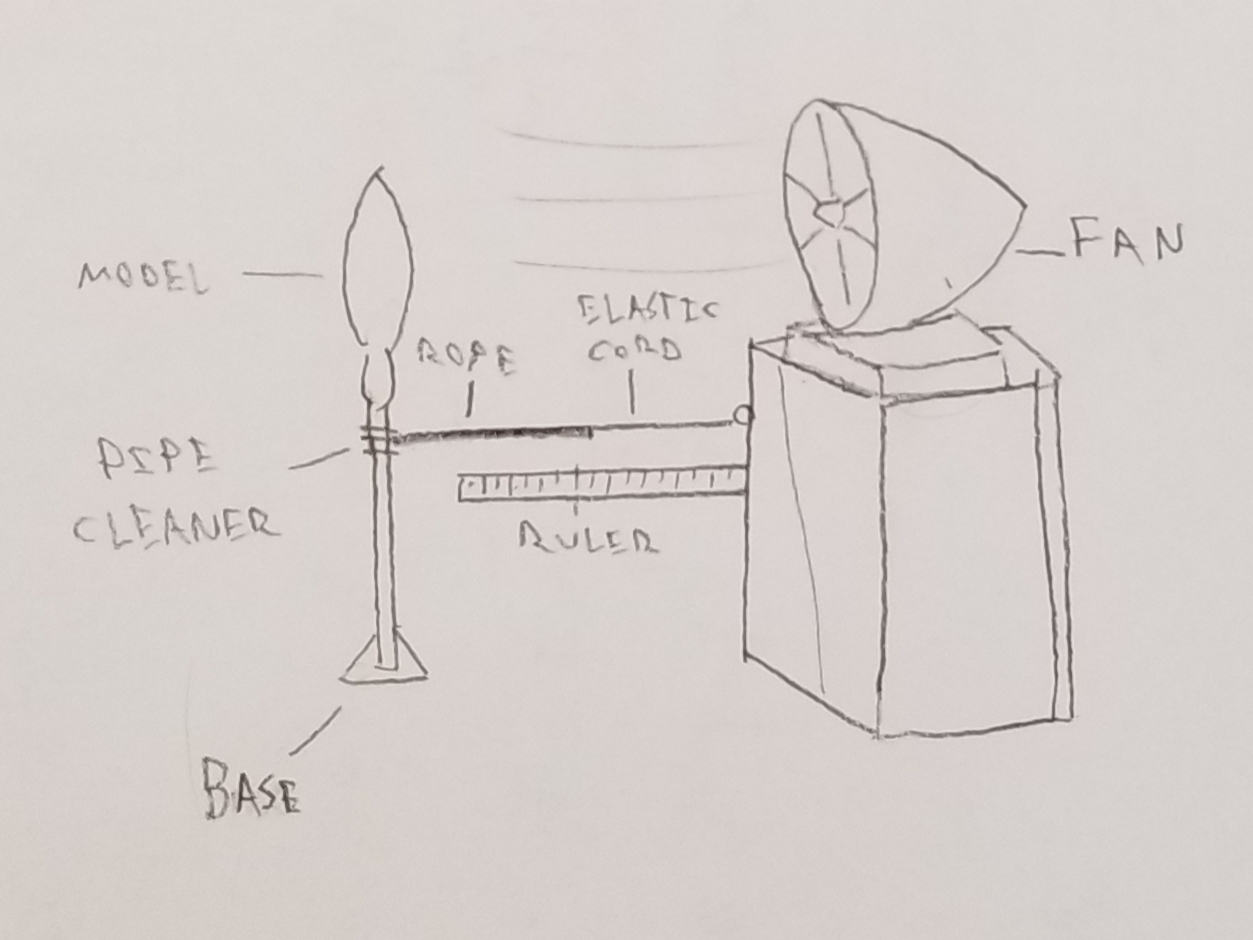
\includegraphics[width=0.5\columnwidth]{figures/Setup2.jpg}
\end{center}
\caption{The setup for testing the rigid model drag when exposed to wind.}
\label{fig:methods3}
\end{figure}




\subsection{Specimens and physical models}
I used a single \SI{6}{y} old specimen of \Citrusxparadisi\ (grapefruit) for all measurements. This specimen was germinated in Toledo, Ohio in January of 2014. As it grew, it spent its summers in the bright outdoors and winters in the relatively dark indoors, staying in a plastic pot throughout its life. This caused it to grow top heavy, with larger leaves in the canopy and smaller leaves in its understory. Additionally, it was subject to attacks from Tetranychid mites each winter, leaving many leaves scarred. At the time of these trials, the specimen had just ended its winter indoor period, causing it to experience rapid growth. It stood at \SI{41}{in} tall and measured \SI{25}{in} across at its widest point. The wind tunnel analysis was focused on the plant's disproportionately large top.

To remove the effects of flexibility, I also created a physical model of a single \Cxparadisi\ leaf using \SI{0.1}{\milli\meter} thick aluminum sheeting from a food container (Chipotle; 6658 Airport Hwy ste c, Holland, OH 43528). To prepare the physical model, I traced an actual leaf and cut the profile of the model to match. The physical model was mounted on a wooden pencil to provide a rigid attachment point compared to the typical flexible leaf petioles on \Cxparadisi. The finished product can be seen in \fref{fig:methods2}.

\subsection{Statistical analyses}
Statistical analyses of the effects of both leaf and fan speed on drag and drag/area were performed using R \citep{r2020} using two-way analysis of variance (ANOVA); plots were prepared using the \lstinline{tidyverse} and \lstinline{ggplot2} libraries \citep{wickham2019tidyverse}.

Applying the percent difference formula

\[D=100*\frac{2*|V1-V2|}{|V1-V2|}\]
yields a difference of 17 percent between the drag to area ratios of the model and the actual plant at fan setting 3. 








 %\section{Methods and materials}
\section{Results}
\label{sec:results}

\subsection{Area measurements}
Area measurements obtained using color blob detection/segmentation in \Matlab\ are shown in \fref{tab:results:area}.
\begin{table}
\caption{Area normal to flow for \Cxparadisi\ specimen and rigid physical model of a single grapefruit leaf.}
\label{tab:results:area}
\begin{center}
\begin{tabular}{cc}
\toprule
& area, \si{\meter\squared} \\
\midrule
\Cxparadisi\ grapefruit specimen & 0.223 \\
rigid physical model of leaf (metal) & 0.0346 \\
\bottomrule
\end{tabular}
\end{center}
\end{table}






\subsection{Drag measurements}
\Fref{tab:results:displacement} gives the measured raw displacement data for the \Cxparadisi\ specimen and the rigid physical model of a single grapefruit leaf. The resulting drag estimates are summarized in \fref{tab:results:drag} and figures~\ref{fig:results:drag} and \ref{fig:results:dragarea}. \Fref{fig:results:drag} shows... (what does it show). When the drag is normalized by area, the effect of leaf flexibility is apparent. \Fref{fig:results:dragarea} shows... (what does it show). 

\begin{table}
\caption{Measured raw displacement (\si{\meter}) for \Cxparadisi\ grapefruit specimen and rigid physical model of a single leaf (metal).}
\label{tab:results:displacement}
\begin{center}
\begin{tabular}{cccc}
\toprule
grapefruit & grapefruit & grapefruit & metal leaf \\
speed 1 & speed 2 & speed 3 & speed 3 \\ 
\midrule
%0.156 & 0.250 & 0.313 & 0.200 \\ % inches / cm 
%0.188 & 0.188 & 0.250 & 0.0500 \\
%0.250 & 0.250 & 0.313 & 0.100 \\
%0.188 & 0.219 & 0.313 & 0.200 \\
%0.188 & 0.250 & 0.313 & 0.150 \\
0.00397 & 0.00635 & 0.00794 & 0.00200 \\ % convert all to SI units
0.00476 & 0.00476 & 0.00635 & 0.00050 \\
0.00635 & 0.00635 & 0.00794 & 0.00100 \\
0.00476 & 0.00556 & 0.00794 & 0.00200 \\
0.00476 & 0.00635 & 0.00794 & 0.00150 \\
\bottomrule
\end{tabular}
\end{center}
\end{table}

\begin{table}
\caption{Summary of drag estimates for \Cxparadisi\ grapefruit specimen and rigid physical model of a single leaf (metal).}
\label{tab:results:drag}
\begin{center}
\begin{tabular}{lcccc}
\toprule
& grapefruit & grapefruit & grapefruit & metal leaf \\
& speed 1 & speed 2 & speed 3 & speed 3 \\
\midrule
drag, \si{\newton} & \num{0.051\pm0.008} & \num{0.061\pm0.007} & \num{0.079\pm0.007} & \num{0.014\pm0.007} \\
drag/area, \si{\newton\per\meter\squared} & \num{2.4\pm0.4} & \num{2.9\pm0.3} & \num{3.7\pm0.3} & \num{4.5\pm2.1} \\
\bottomrule
\end{tabular}
\end{center}
\end{table}

\begin{figure}
\begin{center}
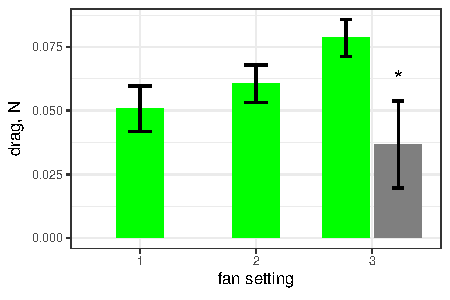
\includegraphics{data/results1.pdf}
\end{center}
\caption{Drag (mean$\pm$sd) for \Cxparadisi\ grapefruit specimen (green) and metal rigid physical model (gray) at different fan speeds. The rigid physical model leaf has less drag than the intact \Cxparadisi\ specimen because of smaller area (two-way ANOVA, $p<\num{4.6e-10}$, $n=5$).}
\label{fig:results:drag}
\end{figure}

\begin{figure}
\begin{center}
\includegraphics{data/results2.pdf}
\end{center}
\caption{Drag, normalized by area, (mean$\pm$sd) for \Cxparadisi\ grapefruit specimen (green) and metal rigid physical model (gray) leaves at different fan speeds. Normalized by area, the rigid metal leaf 19\% more drag than the flexible grapefruit leaves at the same speed, however, the differences are not statistically significant consider the small number of replicates and measurement noise (two-way ANOVA, $p=0.3207$, $n=5$). Differences in drag on the \Cxparadisi\ specimen are apparent at different speeds ($p=0.025$).}
\label{fig:results:dragarea}
\end{figure}






\subsection{Leaf movement during flow}
% This bit needs some help. 
\Fref{fig:results:leafmovement} shows frames from the slow motion video of \Cxparadisi\ at fan speed 3. Following the leaves indicated by the number 1, the leaves which were struck head-on by the wind flexed quite far at their joints, exposing roughly half of their surface area to the camera. The leaf indicated with the number 2 in \fref{fig:results:leafmovement} shows the continued vortex shedding on the leaves when wind was blown across them. The leaf pivoted at its joint, but only exposed about half of its area to the wind before returning to its previous state.
\begin{figure}
\begin{center}
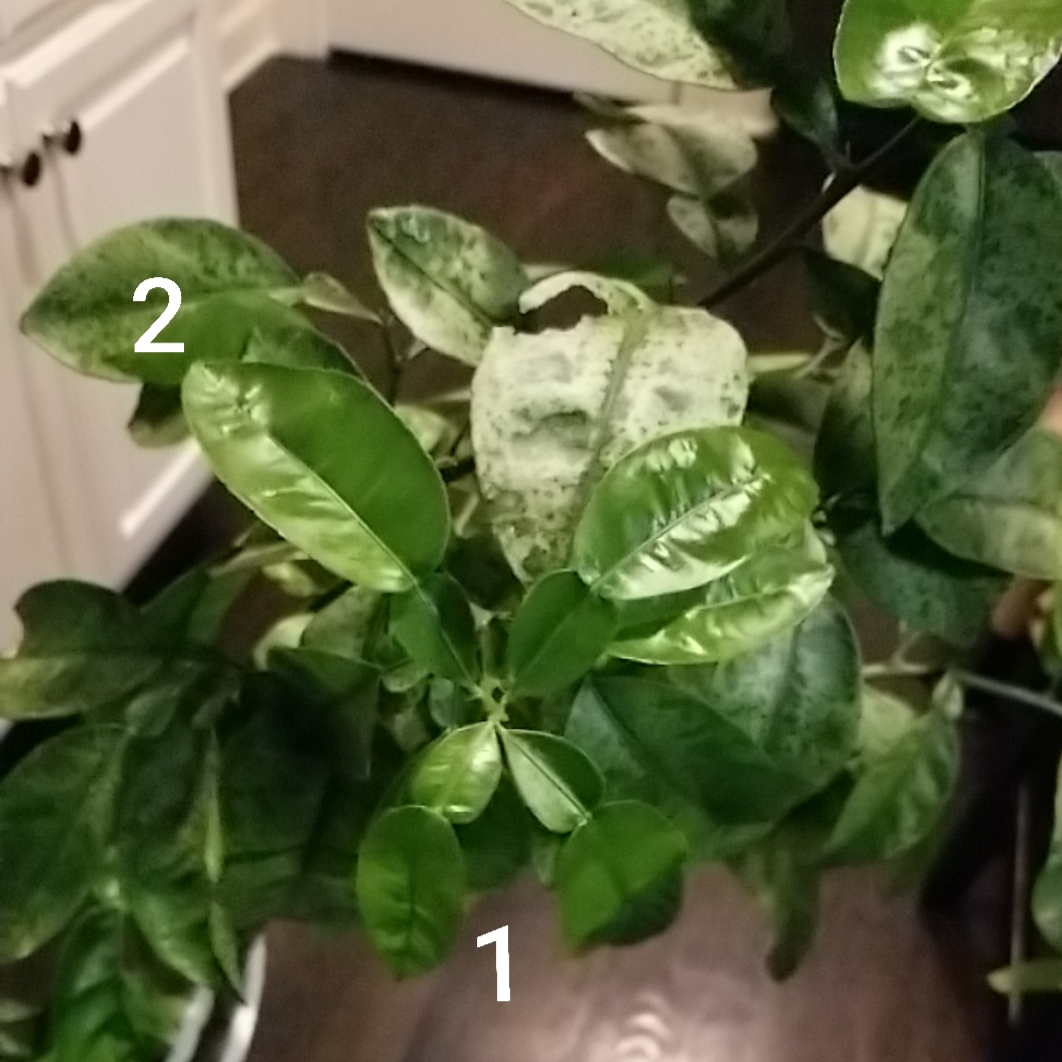
\includegraphics[width=0.49\columnwidth]{figures/Snapshot1.jpg}
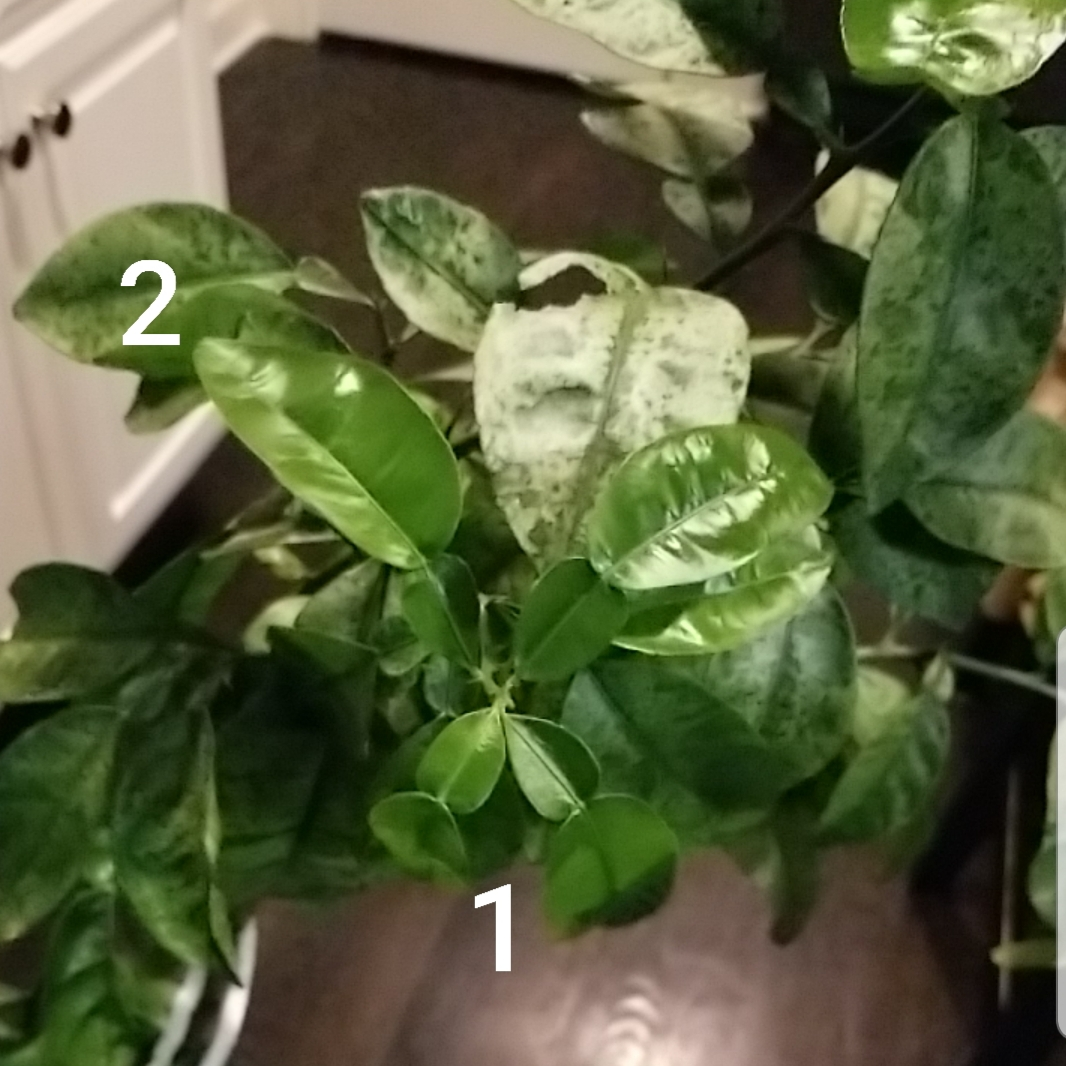
\includegraphics[width=0.49\columnwidth]{figures/Snapshot2.jpg}\\
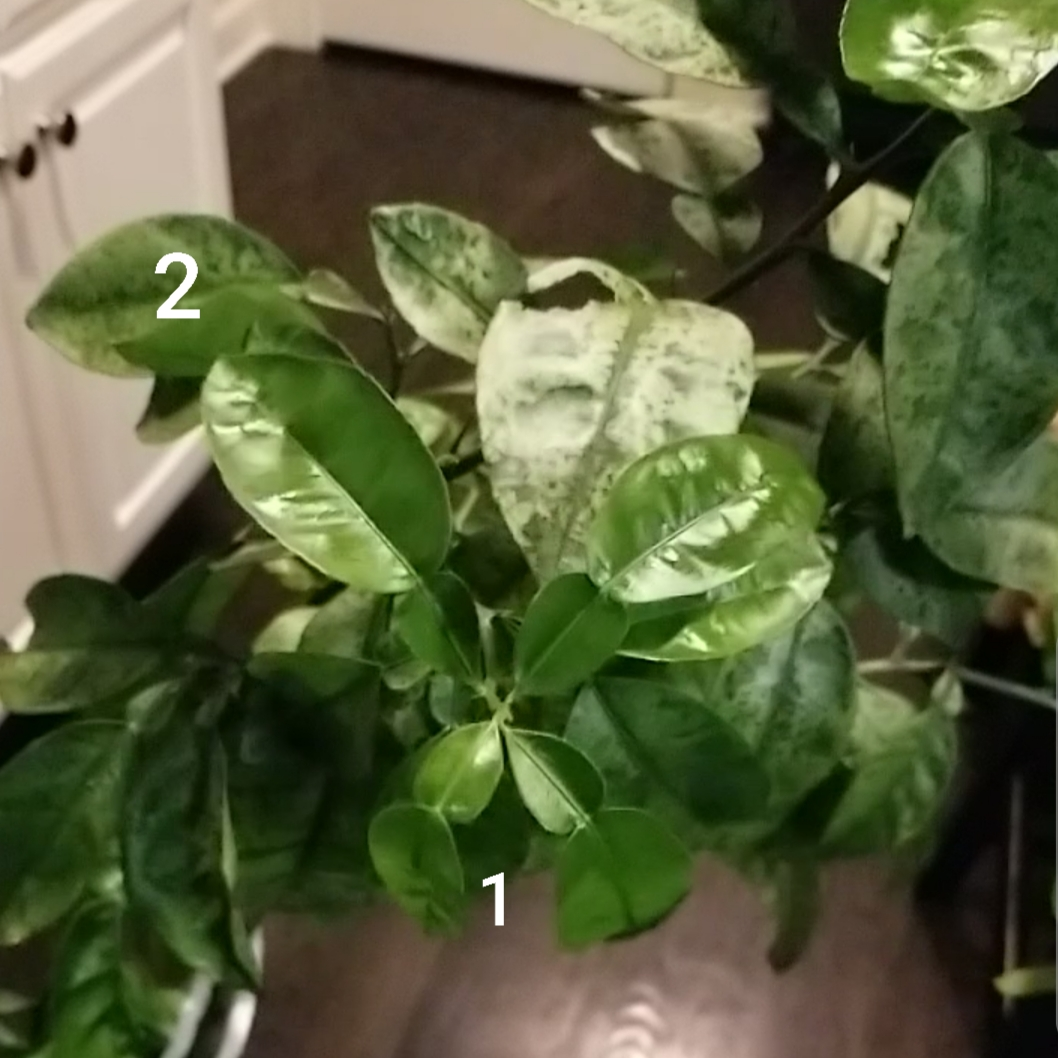
\includegraphics[width=0.49\columnwidth]{figures/Snapshot3.jpg}
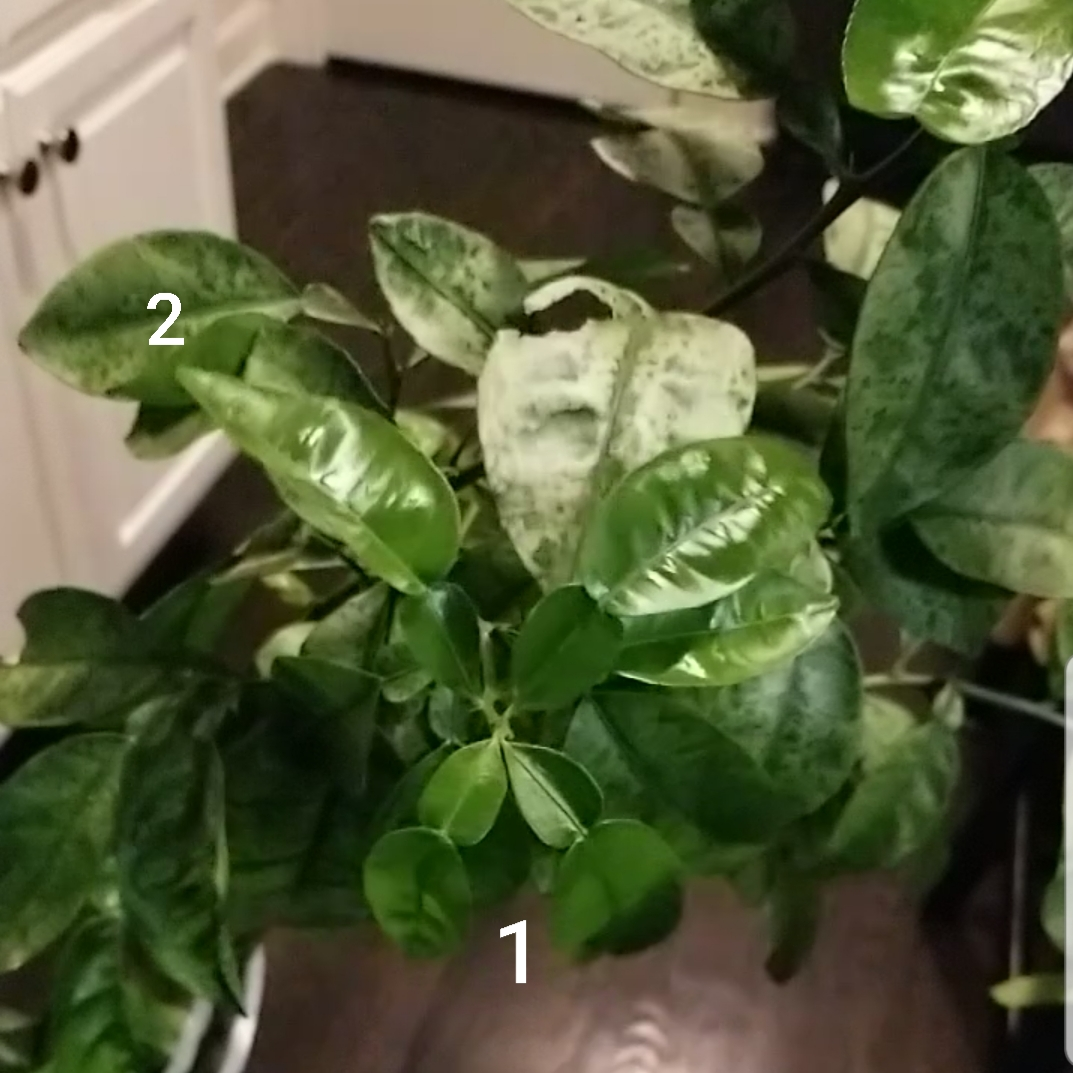
\includegraphics[width=0.49\columnwidth]{figures/Snapshot4.jpg}
\end{center}
\caption{Example frames from slow motion video of \Cxparadisi\ specimen at fan speed 3. Leaves marked 1 and 2 rotate at the petiole, reducing by half their area normal to the flow.}
\label{fig:results:leafmovement}
\end{figure}

 %\section{Results}
\section{Discussion}
Here discuss what your results mean. Are your hypotheses supported or not? Do you have an answer to your overall research question?

 %\section{Discussion}

\section{Acknowledgements}
I thank John Trombetta, Alexis Pak, and Sofia Figueroa for their assistance as classmates in EW282D / EW496. USNA Biomechanics is supported by Lockheed Martin. 

% References
\bibliography{smith.bib}

\clearpage
\appendix
\renewcommand{\figurename}{Supplementary Figure}
\renewcommand{\thefigure}{S\arabic{figure}}
\section{Detailed image processing methods}
\label{sec:A}

Four red-green-blue (RGB) color images (\fref{fig:app:images}) were taken using a Samsung S8 smartphone camera: (1) the orange construction paper with the metal rigid physical model of a single leaf; (2) the orange construction paper alone; (3) the fan aperture alone with black construction paper mask on a blue background; and (4) the fan aperture obstructed by the live \Cxparadisi\ grapefruit specimen. Black and orange construction paper were chosen to maximize contrast and allow easy automatic color segmentation. 
\begin{figure}
\begin{center}
\includegraphics[width=0.49\columnwidth]{figures/MetalLeaf.jpg}
\includegraphics[width=0.49\columnwidth]{figures/Paper.jpg} \\
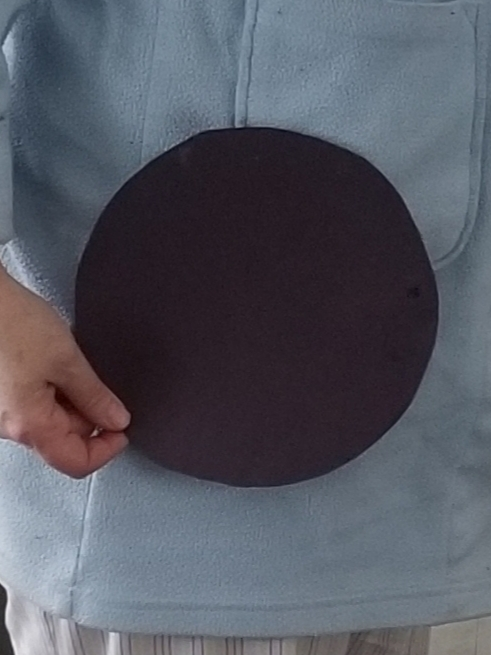
\includegraphics[width=0.49\columnwidth]{figures/Fan1.jpg}
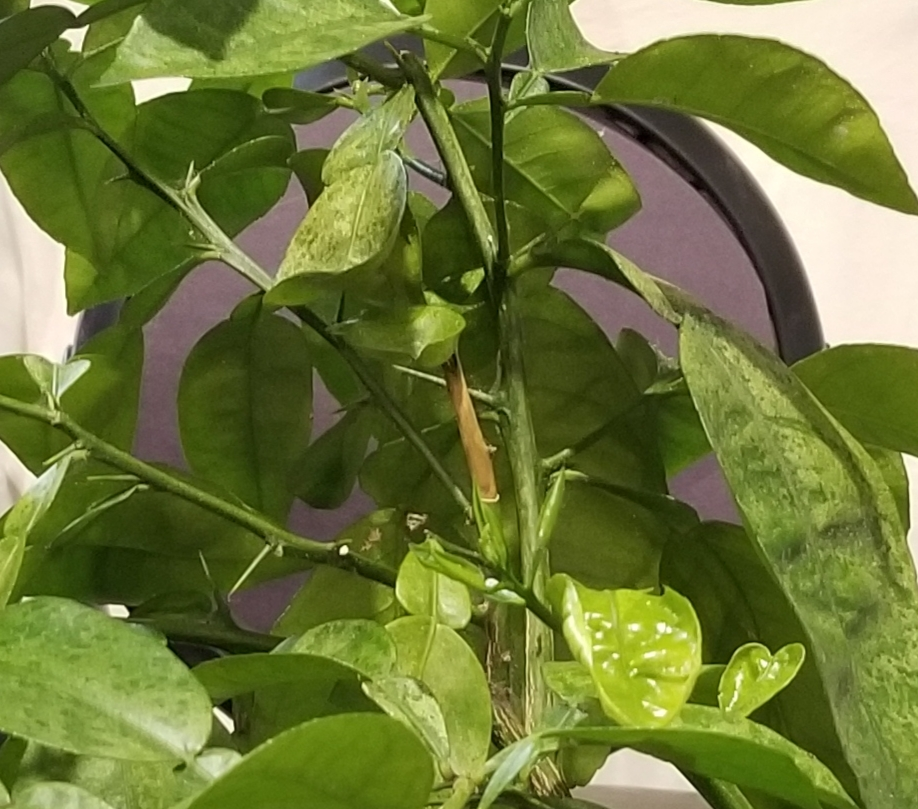
\includegraphics[width=0.49\columnwidth]{figures/Fan.jpg}
\end{center}
\caption{(A) Metal rigid physical model of a leaf on orange background; (B) orange background; (C) fan aperture; (D) fan aperture obstructed by the live \Cxparadisi\ specimen.}
\label{fig:app:images}
\end{figure}


\subsection{Color blob detection/segmentation using \Matlab}
Color blob detection/segmentation was obtained using the \lstinline{colorThresholder} tool in \Matlab. Images were first converted from RGB colorspace to hue-saturation-value (HSV) colorspace; thresholding was then applied in each channel using the sliders to obtain a binary image corresponding to (1) the fan; (2) the area of the fan obstructed by the plant; (3) the orange sheet; and (4) the area of the orange sheet obstructed by the metal leaf, respectively. 

\subsection{Area calculation}
The binary images were labeled as contiguous regions using the \lstinline{bwlabel} command; the largest blobs were manually selected for futher processing. From the labeled region, the \lstinline{regionprops} command was used to obtain the \lstinline{FilledArea} property, which corresponds to the number of pixels contained in the selected blob. 

Using known dimensions of the paper, the area of leaves could be found by calculating the ratio of exposed to unexposed paper area. In the case of the orange construction paper, the paper physical dimensions were \SI{9x12}{\inch} (\SI{0.229x0.305}{\meter}). In the case of the fan, the disk area was \SI{8.5}{\inch} (\SI{0.216}{\meter}) in diameter; these provided the scaling between pixel area and physical area:
\begin{lstlisting}
paperarea=9*12/144;
blackarea=8.5^2*pi/(4*144);
metalarea=leafsize.FilledArea/papersize.FilledArea*paperarea;
grapefruitarea=blackarea-blackarea*fansize/fan1size.FilledArea;
\end{lstlisting}

Area analysis code is provided in the file \lstinline{data/matlab/Calculating Areas.m} in the Github repository at:\\ \url{https://github.com/ew282d-evangelista/ew282d-sp2020-0451-smith}. 




\end{document}
